%!TEX root = ../construction.tex
% -*- root: ../construction.tex -*-

\section{Experimental Result}

제안하는 시스템의 사용성과 효율성을 검증하기 위하여 사용자 테스트를 수행하였다. 실험은 \cite{yeh_-site_2012,lin_using_2014}를 참고하여 설계되었다.

\subsection{Demo Case}




\subsection{Experiments Design}

% 총 30~36명의 피실험자가 실험에 참여하였다. 이중 x명은 여자였고 x명은 남자가 참여했으며, 나이는 26세부터 43세까지이다. 피실험자의 x명은 civil engineering background이고 x명은 (construction professionals with experience in computer aided engineering, software development, structural analysis and design, construction planning, construction drawing, and project management.) 이들 대부분은 도면에 대한 이해도가 높고 CAD 프로그램에 대한 경험이 많았고, 또한 kinect등 제스처 기반 시스템에 대한 경험은 없었다. 

피실험자 설명 관련 설명: 인원, 성별 및 나이 구성, background

실험은 초반 15분 동안 demonstration session을 진행하였다. demonstration session 동안, 전체 시나리오에 대한 비디오를 보여준 후, 제안하는 시스템의 사용 방법에 대하여 설명하고, 나머지 시간 동안 실제로 사용해 본 수 있도록 하였다. 이후에 비교 실험과 사용성 평가를 실시하였다. 비교 실험은 \cite{yeh_-site_2012}과 마찬가지로 제안하는 시스템과 대조군 시스템 사이의 비교실험을 적용하여 몇 가지 과제를 수행하도록 하고 수행시간을 비교하였다. 모든 실험은 비디오로 녹화되었으며, 녹화된 동영상 분석을 통하여 수행시간을 측정하였다. 

대조군에 대한 설명 (paper 기반, 모바일, 제안하는 시스템)
모바일 앱
 - Autodesk® BIM 360 Glue
 - BIMx 

비교 실험에 수행된 과업은 \cite{yeh_-site_2012}와 유사하게 설계하여 실제 건축 환경에서 문제가 되는 task를 반영하였다. 이는 건축 현장에서 건축물의 정보를 획득하고 이를 다시 건축 모델에 반영하는 일련의 과정을 반영하고 있다. 세부적인 task는 아래와 같다. 각 task는 독립적으로 수행되었으며, 새로운 task 수행 전에 5분간의 휴식 시간을 제공하였다. 실험은 이러한 각 task의 수행 시간을 측정하였다. 
Random하게 수행하게 함

\begin{enumerate}
\item Exploration: 3차원 모델을 돌려보고 특정 뷰에 있는 특징 발견하기
\item Query: 특정 층의 특정 평면도 획득
\item Legend: 건축물의 평면도에서 특정 구조물의 dimension 획득
\item Modify: 건축물의 평면도에서 특정 구조물을 다른 위치로 이동됨을 표시
\item Discussion: 원격의 관리자와 건축물의 특정 위치의 이슈 에 대하여 의견 교환
\end{enumerate}

\begin{figure}[ht!]
	\centering
    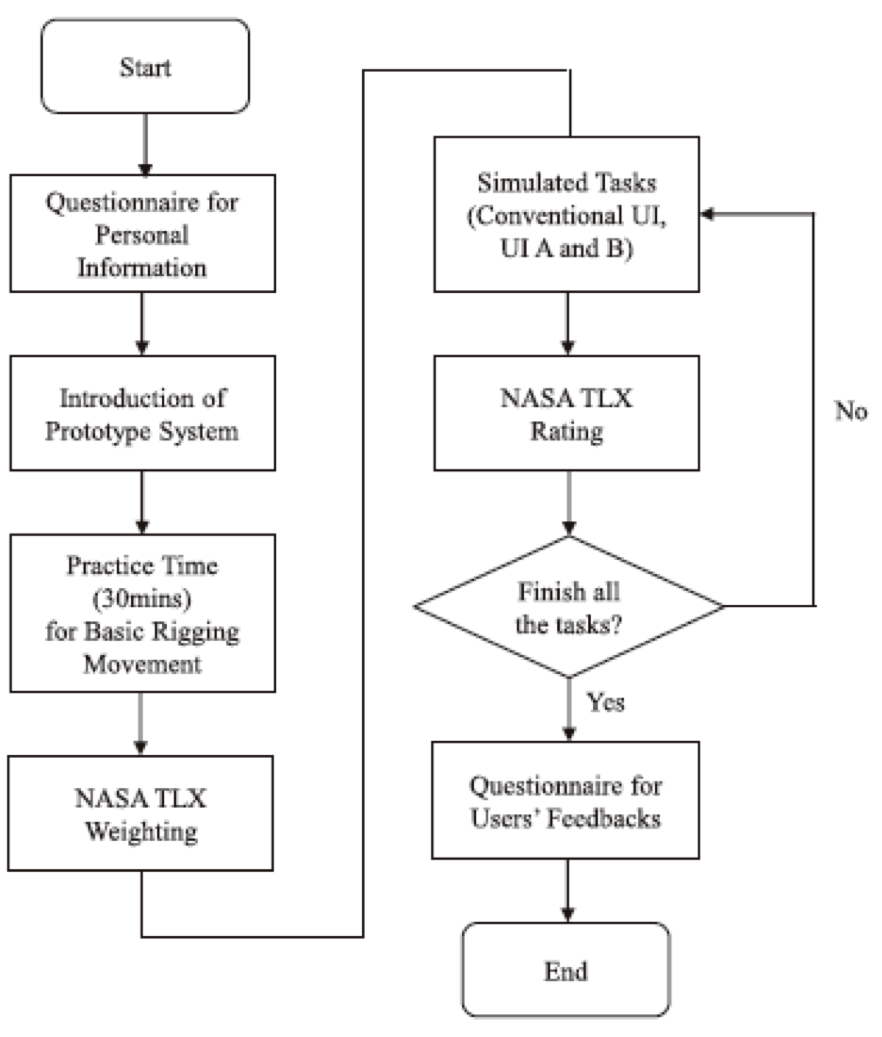
\includegraphics[width=0.4\textwidth]{5-Experiments/process}
	\caption{The process of experiments}
    \label{fig:exp_process}
\end{figure}

\ref{fig:exp_process} 와 같은 형태로 실험 단계 수행

\subsection{Efficiency}

Completion time, success rate test

\subsection{effectiveness}
Task loading score for participants (NASA Task Load indeX) test

\textit{
\begin{itemize}
\item Six weighted factors (Mental Demands, physical demands, temporal demands, effort, performance, frustration)
\item Mental Demand: How much mental and perceptual activity was required? Was the task easy or demanding, simple or complex?
\item Physical Demand: How much physical activity was required? Was the task easy or demanding, slack or strenuous?
\item Temporal Demand: How much time pressure did you feel due to the pace at which the tasks or task elements occurred? Was the pace slow or rapid?
\item Overall Performance: How successful were you in performing the task? How satisfied were you with your performance?
\item Frustration Level: How irritated, stressed, and annoyed versus content, relaxed, and complacent did you feel during the task?
\item Effort: How hard did you have to work (mentally and physically) to accomplish your level of performance?
\end{itemize}
}

\begin{figure}[ht!]
	\centering
    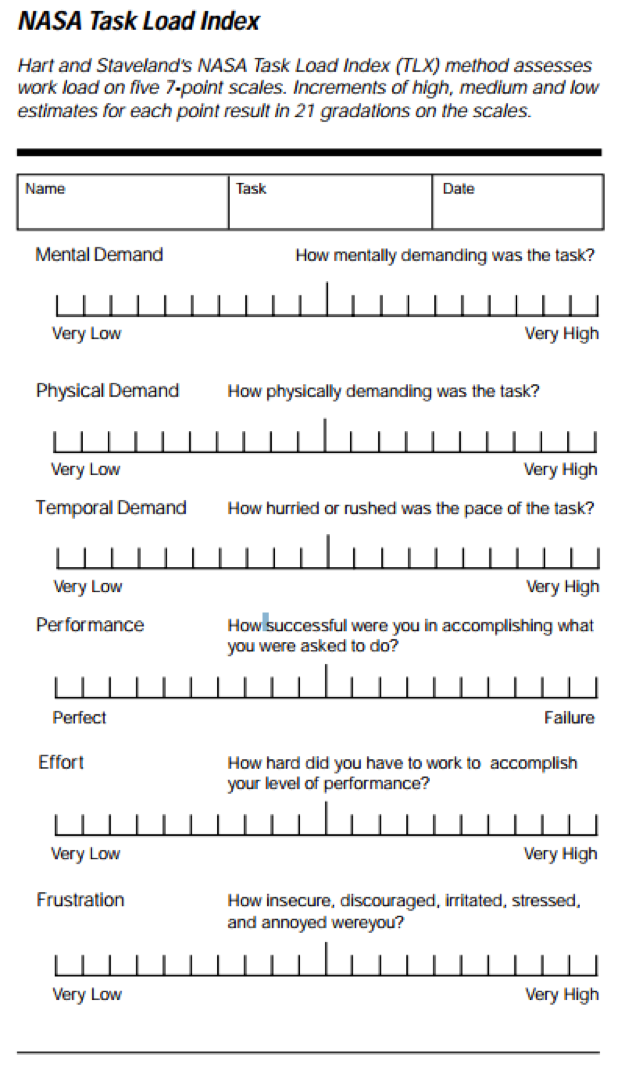
\includegraphics[width=0.4\textwidth]{5-Experiments/NASATLX}
	\caption{Questionnaire of NASA TLX}
    \label{fig:nasa_tlx}
\end{figure}

\subsection{usability}

Usability test (Perceived Usefulness and Usability)



